\section{Projekt i implementacja aplikacji}

\subsection{Diagram przypadków użycia}

Funkcje aplikacji, czyli diagram przypadków użycia przedstawia rysunek \ref{rys:przypadki}. Wszystkie z wymienionych funkcjonalności zostały zrealizowane.

\begin{figure}[H]
	\centering
	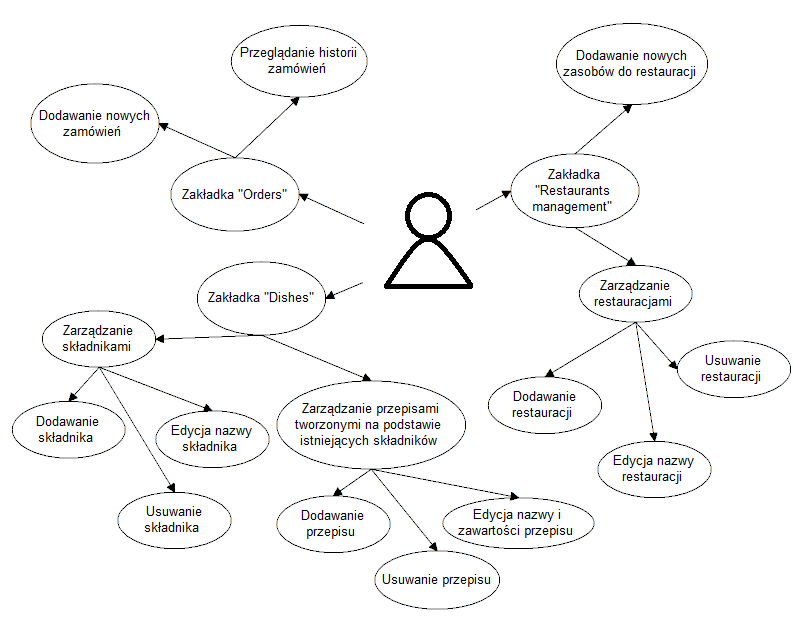
\includegraphics[width=\textwidth]{przypadki}
	\caption{Diagram przypadków użycia}
	\label{rys:przypadki}
\end{figure}



\subsection{Realizacja funkcjonalności}

Aplikacja została zrealizowana w technologii ASP.NET MVC.w środowisku Visual Studio 2015. Poniżej znajdują się przykłady kodu realizującego funkcje wzorca MVC: modelu, kontrolera i widoku, a także klasa DbContext, odpowiadająca za połączenie z bazą danych oraz klasa GenericDataService, która używa DbContext. Warto wspomnieć, że dwie ostatnie klasy zostały napisane w sposób generyczny, co oznacza, że nie trzeba było powielać implementacji dostępu do bazy danych dla każdej kolekcji z osobna.\\
Należy zaznaczyć, że baza MongoDB, jako baza dokumentowa, zamiast klasycznych tabel posiada kolekcje dokumentów. W przypadku zapisywania elementu kolekcji, która nie istnieje, zostaje ona utworzona.

\begin{figure}[H]
	\centering
	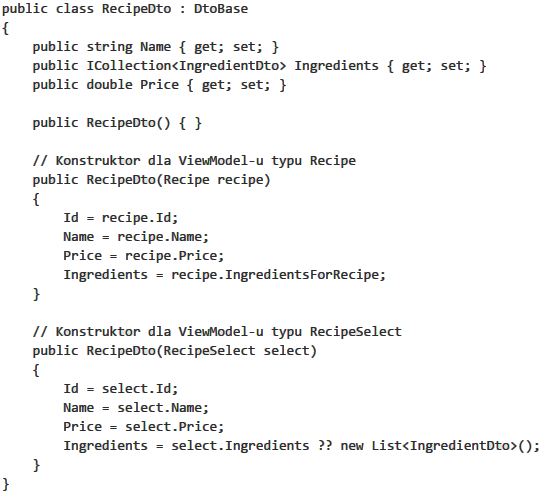
\includegraphics{model}
	\caption{Model na przykładzie \textit{RecipeDto}}
	\label{rys:model}
\end{figure}

\begin{figure}[H]
	\centering
	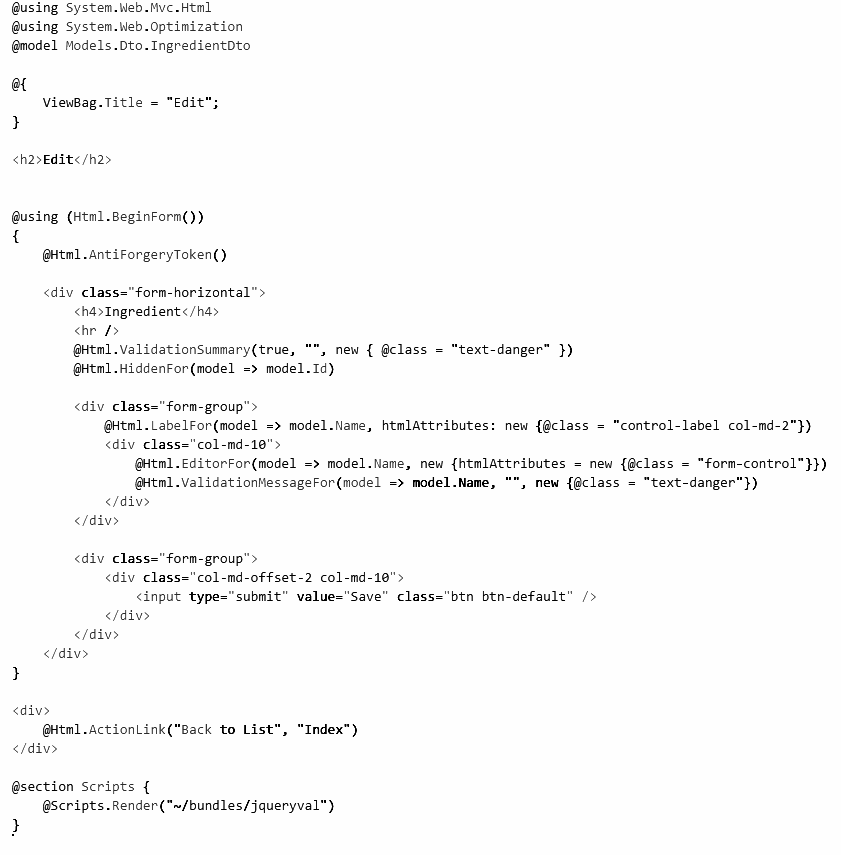
\includegraphics[width=\textwidth,height=0.9\textheight]{view}
	\caption{Widok edycji dla IngredientsDto}
	\label{rys:view}
\end{figure}

\begin{figure}[H]
	\centering
	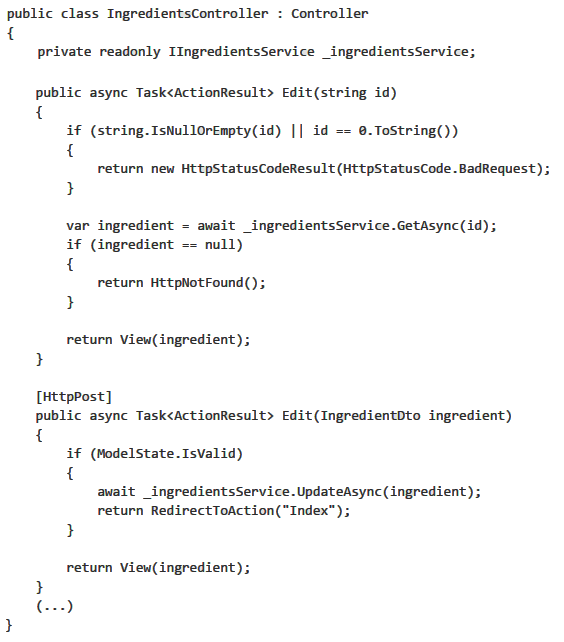
\includegraphics{controller}
	\caption{Kontroler dla kolekcji Ingredients - metody edycji}
	\label{rys:controller}
\end{figure}

\begin{figure}[H]
	\centering
	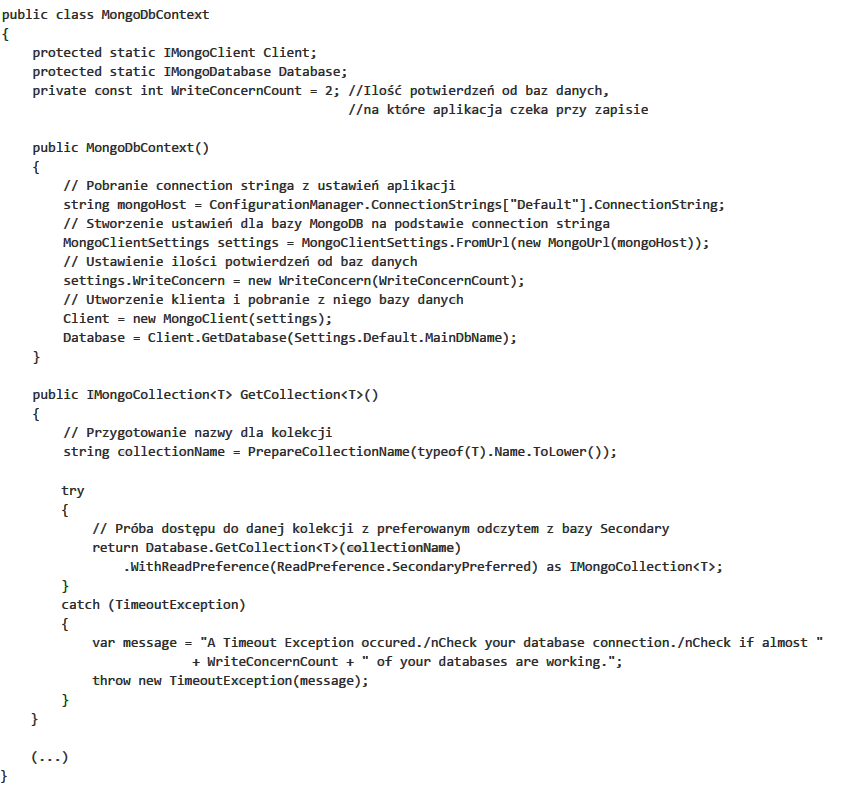
\includegraphics[height=0.8\textheight]{dbcontext}
	\caption{Klasa DbContext - bezpośrednie połączenie z bazą danych}
	\label{rys:dbcontext}
\end{figure}

\begin{figure}[H]
	\centering
	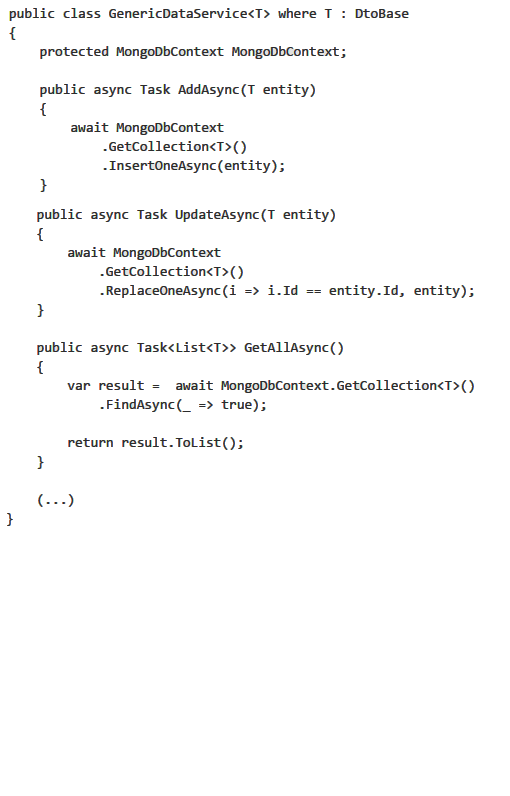
\includegraphics[height=0.8\textheight]{dataservice}
	\caption{Klasa GenericDataService - operacje \textit{dodaj}, \textit{zmodyfikuj} i \textit{pobierz kolekcję}}
	\label{rys:dataservice}
\end{figure}